%Signale

\subsection{Sende- und Empfangssignale}
\label{subsec:Signale}

Dieses Unterkapitel behandelt die theoretischen Grundlagen zum Thema Sende- und Empfangssignale. Ziel ist es, einen realistischen Datensatz zu erzeugen, der dem Signalprozessor zur Weiterverarbeitung zur Verfügung gestellt werden kann. Wir wollen also ein konkretes Simulationsszenario vorgeben können und daraus einen Datensatz (in Form einer Matrix \(M_0)\) generieren, der den realen Gegebenheiten möglichst nahe kommt. Zu einem solchen Simulationsszenario gehören beispielsweise die Anzahl der Ziele im Sichtfeld des Radars (mit deren Radialgeschwindigkeit und Entfernung zum Radar), wie auch einige Parameter, die die Form des Sendepulses bestimmen.

Wir gehen in dieser Projektarbeit (nach Aufgabenstellung) von linear-fre\-quenz\-mo\-du\-lier\-ten Pulsen aus, das heißt, über die Pulsbreite $ \tau $ verändert sich die Sendefrequenz linear. Exemplarisch soll an dieser Stelle der erste Sendepuls des Burst, sowie dessen Echo für ein sich bewegendes Objekt im Sichtfeld des Radars vorgestellt werden. Ein linear-fre\-quenz\-mo\-du\-lier\-ter Puls hat die Form
% 
\begin{equation}
  s(t) := \exp\left( i \, \pi \, B \, (t - \tau/2)^{2}/{\tau} \right) 
        = \exp\left( i \, \Phi(t) \right), \quad t \in [0, \tau] 
\end{equation}
%
mit der Bandbreite \(B\) und der Pulslänge \(\tau\). Der Frequenzverlauf des Pulses ist demnach gegeben durch
%
\begin{equation}
  F(t) = \frac{1}{2\pi}\frac{\diff \Phi(t)}{\diff t} = \frac{B}{\tau}(t-\tau/2), \quad t \in [0, \tau] \text{.}
\end{equation}
% 
% !!! OPTIONAL !!!
%
%Wählt man beispielsweise $ B = 10^6~\text{Hz} $ und $ \tau = 30 \cdot %10^{-6}~\text{s} $, so ergibt sich der in Abbildung \ref{fig:Sendepuls} %dargestellte Sendepuls und Frequenzverlauf. 
%
%\begin{figure}[H] 
%  \centering
%     \includegraphics[scale=0.8]{images/%Sendepuls_und_Frequenzverlauf.png}
%  \caption{Linear-frequenzmodulierter Puls}
%  \label{fig:Sendepuls}
%\end{figure} 
%
% !!! OPTIONAL !!!
%
Grundsätzlich sind bei den Sende- und Empfangssignalen das \glqq Basisband\grqq ~und das \glqq Hochfrequenzband \grqq ~zu unterscheiden. Wie in Abbildung \ref{fig:Sendepuls} zu sehen ist, wird das Basisband durch die mittlere Frequenz Null charakterisiert. Tatsächlich sendet die Antenne elektromagnetische Wellen aber in einem höheren Frequenzbereich - dem Hochfrequenzband. Dafür wird der Frequenzverlauf des obigen Pulses um eine Frequenz $F_{c}$ (c für \glqq carrier\grqq) angehoben, die als \glqq Sendefrequenz\grqq ~oder \glqq Trägerfrequenz\grqq ~bezeichnet wird. Für den hochfrequenten Sendepuls $\overline{s}$ mit der mittleren Frequenz $F_{c}$ gilt also:
%
\begin{eqnarray}
& \overline{s}(t) &= s(t)\cdot  \exp\left( i \, 2 \pi \, F_{c} \, (t - \tau/2) \right) \\
& &= \exp\left( i \, \Phi(t) + i \, 2 \pi \, F_{c} \, (t - \tau/2) \right) 
\end{eqnarray}
%
für $ t \in [0, \tau] $. Dementsprechend gilt für den Frequenzverlauf
%
\begin{eqnarray}
& \overline{F}(t) &= \frac{B}{\tau}(t-\tau/2) + F_{c} \\
& &= F(t) + F_{c}
\end{eqnarray}
%
für $ t \in [0, \tau] $ . Die Simulation des Exciters ist an dieser Stelle abgeschlossen. Wir widmen uns nun dem Receiver und betrachten dementsprechend die Empfangssignale. Die Form und Position des Echosignals im Zeitbereich hängt im Wesentlichen von zwei Faktoren ab: Dem Abstand zwischen Radar und Ziel und der radialen Geschwindigkeit des Ziels. Um das Empfangssignal zu konstruieren, betrachten wir den Abstand zwischen Radar und Ziel als Funktion $ R(t) $. Wird vom Radar ein Sendepuls $ \overline{s}(t) $ ausgesendet, so lässt sich das Echo $ \overline{r}(t) $ beschreiben durch eine verzögerte Kopie des Sendepulses. Wir erhalten 
%
\begin{eqnarray}
& \overline{r}(t) = c_{mag} \cdot \overline{s}(t - \frac{2 R(t)}{c}) \text{,}
\label{eq:echo}
\end{eqnarray}
%
wobei $ c $ der Lichtgeschwindigkeit entspricht. Der Parameter $ c_{mag} $ dient dazu, die Stärke des reflektierten Signals berücksichtigen zu können (mag für \glqq magnitude\grqq). Dieser hängt beispielsweise von der Größe des Ziels ab. Obige Formel (\ref{eq:echo}) führt nach \cite[Seite 95]{Richards} zu einer korrekten Beschreibung des zeitabhängigen Dopper-Shifts. Geht man von einer Anfangsentfernung $ R_0 = R(t=0) $ und einer konstanten Radialgeschwindigkeit $ v_{r} $ des Ziels aus, dann gilt $ R(t) = R_0 - v_r\cdot t $. Eine positive Radialgeschwindigkeit entspricht dabei einem Ziel, das sich dem Radar nähert. Um das Basisband-Echosignal zu erhalten, verschieben wir den Frequenzverlauf des reflektierten Signals $ \overline{r}(t) $ um $ F_c $ nach unten, also
%
\begin{eqnarray}
& r(t) = \overline{r}(t)\cdot \exp\left(- i \, 2 \pi \, F_{c} \, (t - \tau/2) \right) \text{.}
\end{eqnarray}
%
Dieses Signal $ r(t) $ wird anschließend mit der Sampling-Frequenz  $ S $ abgetastet und in der entsprechenden Zeile der Matrix $ M_0 $ abgelegt. Die i-te Zeile $ (i = 1,...,M) $ der Matrix $ M_0 $ repräsentiert dabei den mit der Rate $ S $ abgetasteten/gesampelten Zeitbereich $ [\tau + (i-1)\cdot \text{PRI}, \enskip i\cdot \text{PRI}] $. Bei den Zeilen von $ M_0 $ spricht man auch von \glqq Slow Time Samples\grqq , während man die Spalten der Matrix als \glqq Fast Time Samples\grqq ~bezeichnet. Nach der Überlagerung der gesampelten Signale (jedes Ziel erzeugt ein Echo), wird noch weißes (d.h. normal verteiltes) Rauschen hinzugefügt. Mit der Matlab-Funktion \texttt{generate\_{}cpi\_{}return\_{}matrix.m} wird die Generierung der Matrix $ M_0 $ realisiert. Sie ist in \cref{chap:Quellcode} zu finden.

Zusammenfassend stellt die folgende Abbildung \ref{fig:ZusFas} schematisch den oben beschriebenen Ablauf von der Generierung des Sendepulses bis zum Abtasten des Basisband-Echosignals dar. 
%
\begin{figure}[H] 
  \centering
     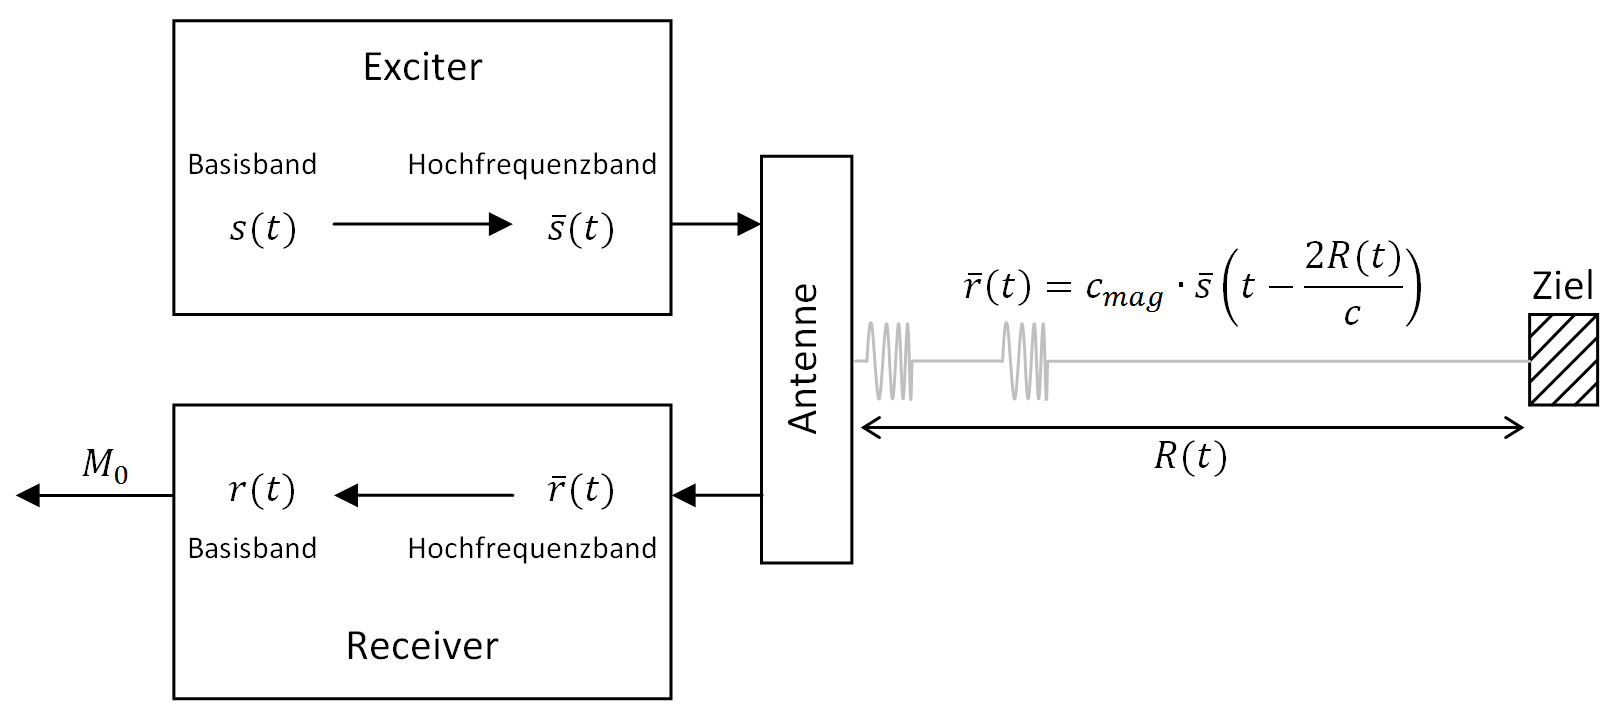
\includegraphics[scale=0.4]{images/Signals_Exciter_Receiver_Zoom240.PNG}
  \caption{Schematische Darstellung des Ablaufs}
  \label{fig:ZusFas}
\end{figure} 
%